\documentclass{scrreprt}
\usepackage{glossaries}
\usepackage{listings}
\usepackage[]{graphicx}

\newglossaryentry{latex}{
  name=LaTeX,
  description={Ein Textsatzsystem}
}
\newglossaryentry{consumer}{
    name=Consumer,
    description={A program using a UaDI conform DLL to get generated data from a producer or device}
}
\makeglossaries

\tableofcontents
\newpage 

\begin{document}

\chapter{The Idea of OmniView}
OmniView is planned to be an omniscient data-visualization and analysis tool. 
OmniView itself shouldn't need to know anything about any given data-producer at compile-time, but should still be able to visualize the produced information.
OmniView itself shouldn't need to know anything about any given analysis-tool at compile-time, but should still be able to use an analysis-API. 
In order for OmniView to work this way, there shall be a structured architectural approach, to enable modular development.
This includes dataproducer devices as well as analysis-tools.

\section[Modules]{Modules of OmniView and their Role}
The Name OmniView actually only applies to the executable instance, that is in charge of displaying gathered data in a way similar to PicoScope or sigrok, whether it's live or archived data. 
Since (well-designed) modularity can help keeping the complexity of a system in check, the greater OmniView-Architecture is a project of the Bochumer AI-Group.
\\
A oscilloscope-like user-interface is the most generic way, to display data as a function over time. 
All measurement-values are a sample of a certain unit (sometimes even an SI-Unit) at a specific point in time, and thus projectable onto a plane with its unit in y- and the time in x-dimension. 
Displaying a multitude of different y-dimensions in an oscillogram is a well-proven design and has been implemented in several data-recorder software-suites. 
\\
Incoming live-data into the view is delivered via a websocket connection.
There won't be hard real-time guarantees in this interface. 
This websocket is provided by an entity that implements the concept of an epoch-server.
Soft real-time can be guaranteed to a certain extend in the internal structure of the epoch-server and its storage-interface.
Due to the nature of live-updates of a GUI, new updates are being received on a regular basis and prepended to the n-1 dataset.
Each update-object that contains data to be prepended, and displayed in the oscillogram is called a column. 
It derives its name from the property, that it holds several values of different data-channels in parallel.
The aggregation to a continuous stream of such pieces of information that belong to one channel is called a waveform. 
\\
An epoch-server has the ability to maintain multiple websocket connections, and an OmniView-Instance has the ability to maintain connections to multiple epoch-servers. 
Before a view can instantiate a connection with a websocket, it queries the epoch-servers REST-API, to receive a structure know as possibility-list.
This list contains all available devices, and all available transducers. 
A transducer is a function that works as a filter.
It implements a directed node, taking one or more waveforms as an input and having exactly one waveform as an output. 
Using transducers, a so-called (processing-)route can be constructed. 
A route is a directed graph composed from transducer-nodes. 
For further investigation see \ref{chap:WaveformProcessingNetwork}.
The structure inside the epoch server that defines which channels are being send out to a specific connection is called the connections visibility-list. 
This list in combination with a checkbox will also be displayed in the view.

\begin{figure}
    \includegraphics[\width=.9]{assets/overview.pdf}
    \caption{Overview of Modules}
\end{figure}

\section[Greater Picture]{OmniView and its Role in the Greater Picture}
Auto-Intern GmbH and their connected entities have been working on a unified architecture for measurement- and monitoring-devices since the early 2000s. 
Integrating measurement-systems into larger architectures is by no means a trivial task.
OmniView fits into the Grand-Unified-Monitoring-Architecture of Auto-Intern.


\begin{figure}
    \includegraphics[width=.9\textwidth]{./assets/pictures/overview.pdf}
    \caption[]{Brief overview of the proposed structure}
    \label{fig:overview}
\end{figure}


There shall be a unified way to interact with an abstract data-producer.
This includes devices such as:
\begin{enumerate}
    \item a USB-oscilloscope \gls{latex}
    \item a TCP/IP client, sending a continuous stream
    \item a USB-logic-analyzer
    \item a random-number-generator
    \item a filedescriptor
\end{enumerate}

Since it is not known at compile-time, which devices will be used at runtime, the code can't be linked statically into OmniView (or any other data-\gls{consumer} for that matter). 
Therefor an interface shall be defined, that gets used by the consumer, but the implementation of the data-handling ought to be provided in a dynamically linked library. 
From here on forward we will refer to this as \lstinline|DLL| even though \lstinline|.dll| and \lstinline|.so| are meant equally. 
If a windows \lstinline|.dll| or a linux \lstinline|.so| is meant specifically, please use the terms \lstinline|.dll| or \lstinline|.so|, otherwise \lstinline|DLL|. 
Be aware, that this \lstinline|DLL| does not necessarily constitue an aquivalent to an actual device-driver with a communication-channel to the systems kernel.
\\
It appears, that all dataproducers that are relevant for OmniView can be abstracted in a certain way, and thus share the same function-calls in a \lstinline|DLL|.
There are three requirements:
\begin{itemize}
    \item Grabbing the next part of the data-stream asynchronusly
    \item The data-producer providing meta-information about itself 
    \item Send control-data from the consumer to the data-producer
\end{itemize}
This interprocess-communication comes with some additional hurdles.

\section{Memory Management Ideology}
Not only does OmniView not know about which devices will be connected at runtime, it also does neither know about the amount of devices that will be attached, nor does it know what data-rate the producers will provide.
Due to this uncertainties, a strongly structured memory allocation ideology needs to be implemented in order to minimize error-prone sections in the applications code.


\section[UaDI]{Unified abstract Data\-producer Interface}
The \textit{Unified abstract Data\-producer Interface} is the protocol that specifies the interprocess\-communication between the con\-sumer and the device, using the \lstinline|DLL|. 

\begin{figure}
    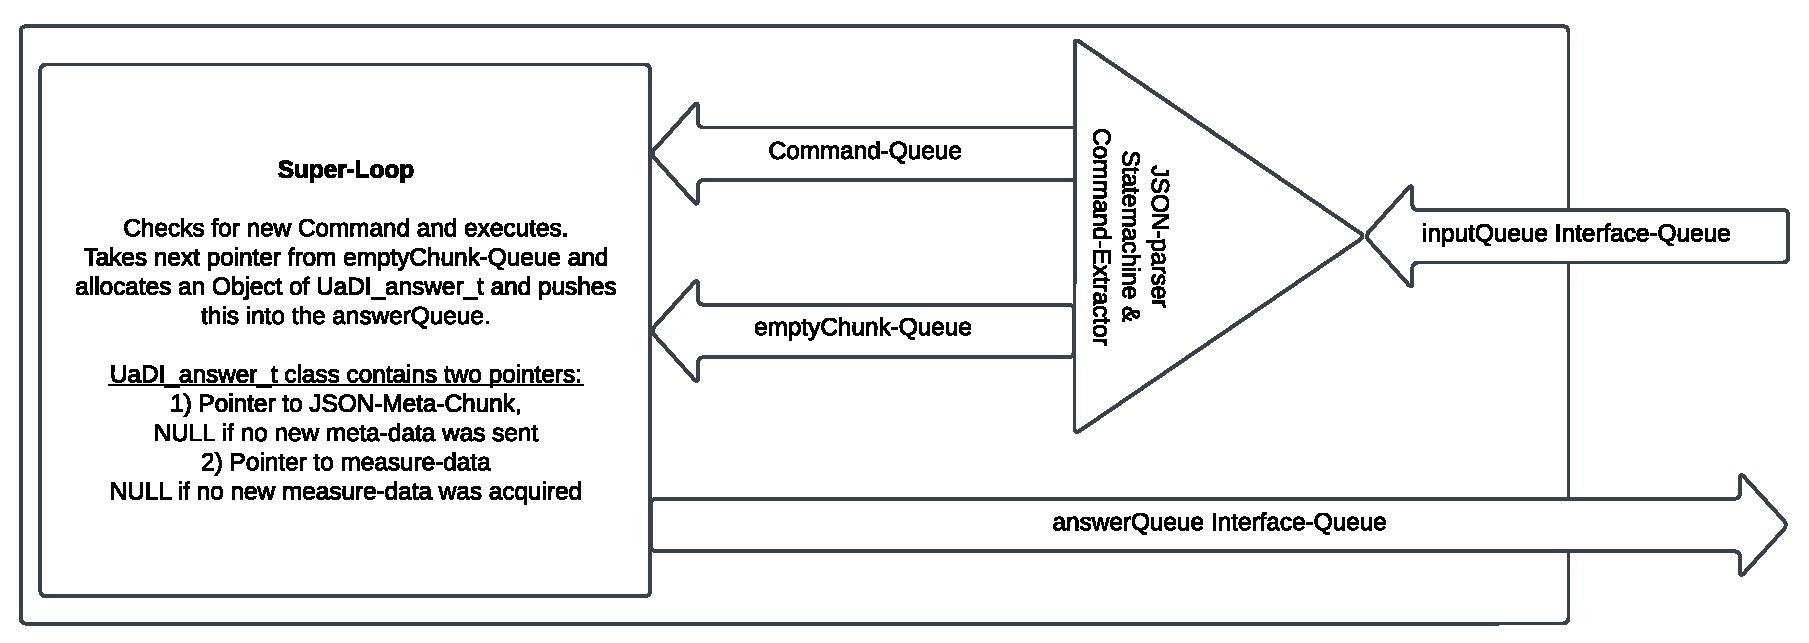
\includegraphics[width=.9\textwidth]{./assets/pictures/interface.pdf}
    \caption[]{Coarse structure of the DLL-interface}
    \label{fig:dllinterface}
\end{figure}


\chapter{Dataproducers}
The origin of a stream of measurement-samples is called a device, as refered to in the UaDI specification. 
A device may get control-input, but always has to back-channels to a consumer:
\begin{itemize}
    \item a pointer to a JSON chunk
    \item a pointer to a data chunk
\end{itemize}
\section{Memory-Management}
A device doesn't allocate on its own.
Therefor it needs to get a memory-pointer from the consumer.
The so called chunks are of a default size of 128*1024 bytes.
Pointer to these memory-locations are known as chunk\_ptr.
The consumer is responsible for the memory management of these chunks.
An array of chunk\_ptr can be handed to the device on claiming it, as well as through a routine called uadi\_push\_chunk.
In both cases, the consumer passes an array of chunk\_ptr, and the amount of chunk\_ptr to the device.
When claiming the device, a callback is also registerd. 
The callback is called, when the device is finished with writing into a chunk.
The callback is called with a chunk\_ptr and a void pointer to the consumers context. 
The device doesn't care about the context pointer, it just hands it back to the consumer.
Which data-type the device hands back is defined by the device. 
In the first usecases, only float shall be supported. 
The data-type will be handled in a second layer on top of UaDI, that performs device-management.

\section{Concrete Devices}
There are several devices already planned that need to be supported by the end of 2024:
\begin{enumerate}
    \item OmniScope - USB-Single-Channel Oscilloscope
    \item OmniScope Duo - USB-Dual-Channel Oscilloscope
    \item OmniEField - USB-E-Field Probe
    \item OmniBField - USB-B-Field Probe
    \item OmniTherm - USB-Thermocoupler Typ-K 
    \item OmniPower - USB-Power-Monitor
    \item OmniPower ETH - Ethernet-Power-Monitor
    \item OmniSonic - USB-Vibration-Sensor
    \item AI PowerProbe - Ethernet E-Field/B-Field Probe 
    \item Random Number Generator Software-Device
    \item IOTA Software Device 
    \item PCIe - Generic Integer Kintex7 FPGA Device
\end{enumerate}


\section{Userinterface}

The following paragraphs describe the Userinterface components and their functionality.
The design of individual components is also introduced here; however, the detailed description of the design principles can be found in Chapter \ref{cap:Designprinciples}. All components should be designed after those principles.\\ 

The user interface is currently implemented in C++; however, there are plans to transition it to JavaScript in a subsequent phase.\\
This interface serves as a central hub for configuring connected devices, conducting measurements, saving data in various formats, displaying and analyzing the acquired data. Additionally, users can access an integrated Help Menu that directs them to a website providing comprehensive information about OmniView and OmniScope.

The basic interface should contain 

\begin{itemize}
    \item a bar at the top where the company name, a saving button, a settings button, a start and stop measurement button are integrated 
    \item an adjustable window where the data is displayed
    \item a side menu which can be minimized for : 
    \begin{itemize}
        \item searching devices 
        \item loading old data 
        \item Diagnostics
        \item Settings
        \item Help
    \end{itemize}
    \item a bottom window which can be minimized where the connected devices and the loaded data files are presented
    \item serveral popup windows that are displayed when using for example a analyses
\end{itemize}

The design can be found in picture \ref{fig: GUI}. 
\begin{figure}[!h]
    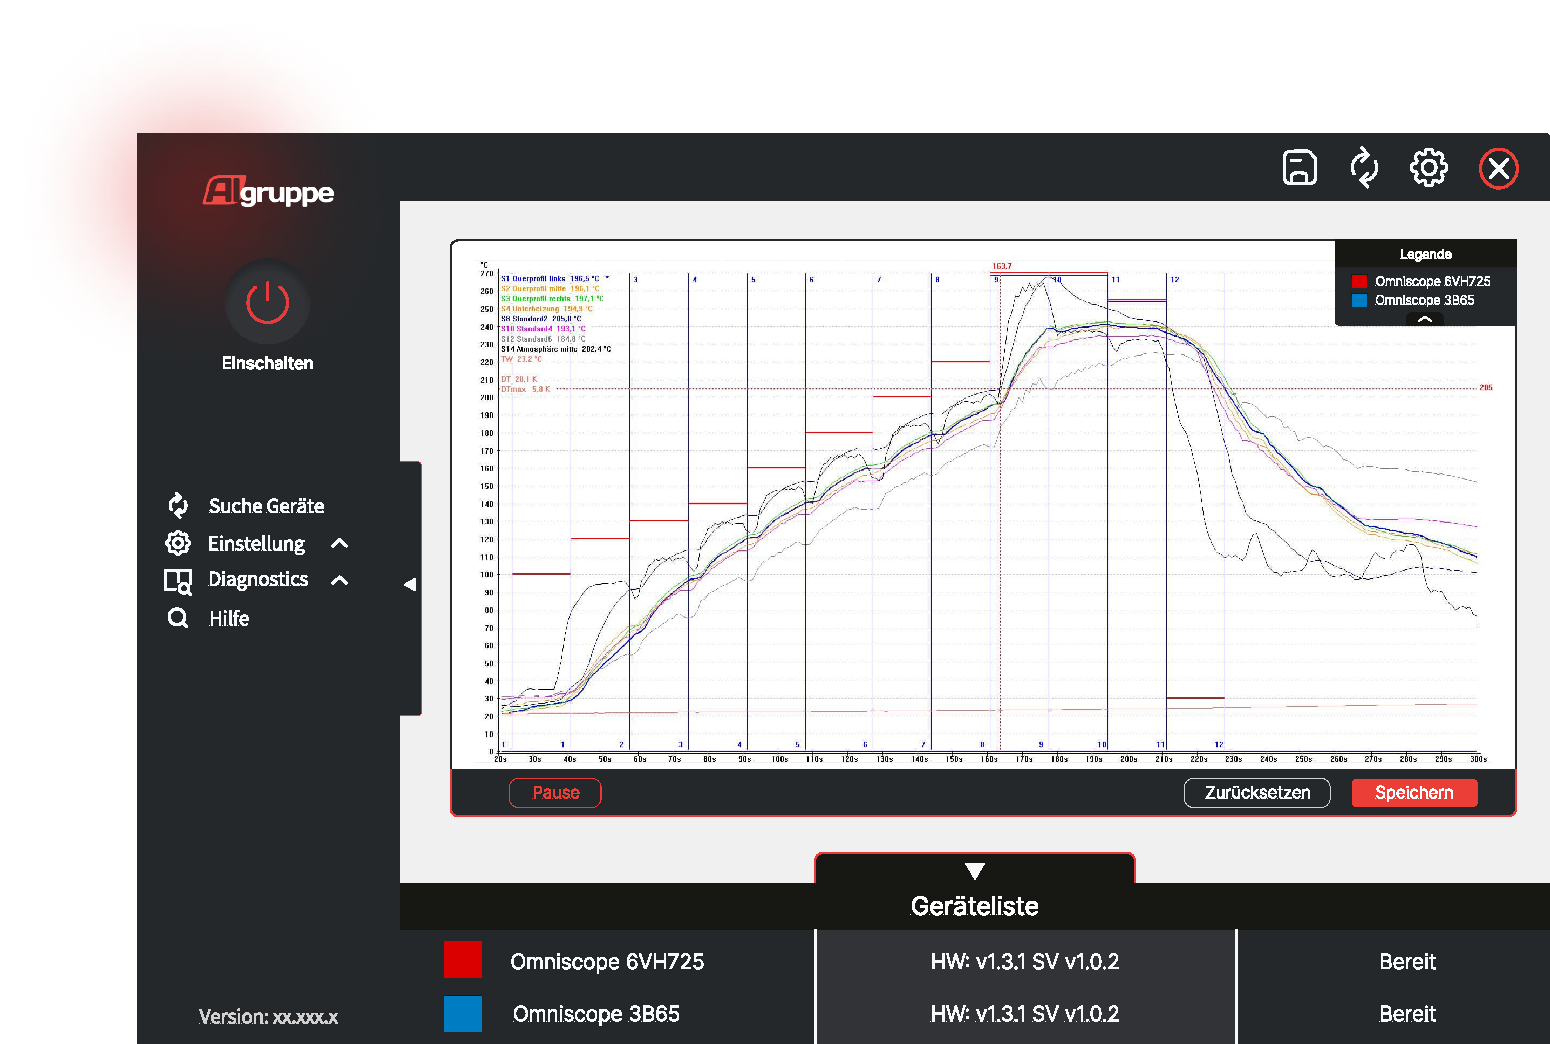
\includegraphics[width= 400px]{assets/pictures/Start Oszi (1).pdf}
    \caption[]{A visual representation of the GUI interface when all menus are selected}
    \label{fig: GUI}
\end{figure}
Right now all buttons are in German, which should be changeable later through the settings menu. 
The size of the GUI should adapt to the size of the respective used screen.

The popup windows will be 
\begin{itemize}
    \item a window to upload the data
    \item a window to save the data 
    \item a window to check the old data analyses results 
\end{itemize}

This popup windows should all follow the same structure and design principles which can be found in the \ref{cap:Designprinciples}. 
An example for a popup window is shown in Figure \ref{fig:PopupwindowDesign}.
This list is not yet completed. 

% insert picture 
The detailed descriptions of the individual components and their functionality is described in the following sections.


\subsection{Toolbar}

The toolbar will be displayed at the top of the programm. 
A picture is shown in figure \ref{fig: toolbar}. 
\begin{figure}
    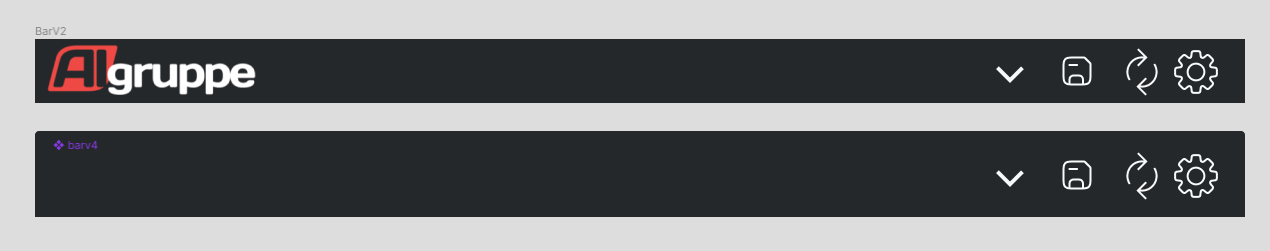
\includegraphics[width=.9\textwidth]{assets/pictures/Toolbar states.png}
    \caption[]{A visual representation of the Toolbar with different buttons}
    \label{fig: toolbar}
\end{figure}
The toolbar contains the company logo at the left side, this logo should only be visible when the side menu is closed. 
At the right side the toolbar contains a save button and a load again/reset button. 
In the middle of the toolbar is a field for starting and stopping the measurements that has different states depending on the current state of the measurement. 

In the following the functionality of the different buttons is descriped. 

\subsubsection{Save button}

The save button should be a Icon button that follows the design principle of the icon button described in chapter \ref{cap:Designprinciples_IconButtons}. 
The save button is used to write the measurement (a waveform stack) into a storage. 
The measurement is defined as a waveform stack because the user is able to save the measurement from only one devices or from many different devices into one or more files.

This section delineates the procedure for transferring the data from a waveform stack or an individual waveform, acquired through the OmniScope, to a storage system via the user interface. The storage options encompass the computer's file system, a Database Management System (DBMS), or a Cloud platform.
%Refer to \cite{fig:saveData} for a visual representation of the corresponding menus.
\\

\textbf{The following describes the User story:} \\

Visibility of Save Button: \\

Prior to initiating the measurement, the save button should be prominently visible.\\

Greyed-out State During Measurement:\\

While the measurement is in progress, the save button should appear in a greyed-out state.\\

Post-Measurement Access:\\

Upon completion of the measurement, users should easily locate and access the now visible save button.\\

Prompt Appearance of Save Window:\\

When the user clicks the save button, a window should promptly appear. This window should be designed after the design principle in chapter \ref{cap:Designprinciples_Popupwindows}\\

Window Components:\\

Within the window, an input field labeled "Speicherpfad" should be positioned in the left corner, accompanied by a "Durchsuchen" button. The buttons should be designed after the design principle in chapter \ref{cap:Designprinciples_PopupWindowButtons}\\

Path Input Options:\\

Users have the option to manually input a path into the "Speicherpfad" field.\\

File-Explorer Integration:\\

By clicking the "Durchsuchen" button, the File Explorer opens, enabling users to manually select a saving path.\\

Default Path Handling:\\

If no path is selected, the system defaults to using Desktop/Omniview/saves/.\\

Visible Default Path:\\

The default path is displayed in the "Speicherpfad" field, appearing greyed out.\\

Device Selection:\\

Users can choose the devices for saving through a dropdown menu under the selected path. The menu should be designed after the design principle in \ref{cap:Designprinciples_dropDownMenusWithCheckmark}.
Only the devices that are connected are shown with their correct device name.
Also files that have been loaded into the devices list are shown.
The number of connected devices is undetermined before the start of the software so their can be multiple devices or just one.\\

Adding Another Path:\\

In cases where multiple devices are connected, users can click a plus button with the description "Speicherpfad hinzufügen" (Add another path) triggering the appearance of another window with identical settings. Here the user also has a "Durchsuchen"-Button where he can choose in which path the data is stored and a drop down menu to choose which devices he wants to be stored in the selected path. The user can also change the name of the measurement.\\

Checkbox Selection:\\

When checkboxes next to the devices are selected, the chosen devices are saved in the same file within the selected directory.\\

Vehicle Information Input:\\

Beneath the "Speicherpfad," four input fields—Vehicle type, VIN, measurement name, and mileage—are available.\\

Dropdown Menu for Vehicle Type:\\

Users can choose the vehicle type via a dropdown menu loaded from a file. The user can only select one vehicle type.\\

Adding Custom Vehicle Type:\\

An option allows users to input a new vehicle type at the end of the dropdown menu, subsequently adding it to the file by clicking a plus button.\\

Final Save Action:\\

Users can initiate the save process by clicking the save button in the right corner, preserving the selected waveform stack in the chosen path as a .csv file. The filename should contain the name of the device and a name set by the user in the "Messung"-field.\\

Information Inclusion in File Name:\\

The information entered about the vehicle ("Messung", "vin", "bekannte Fahrzeuge") should be saved at the top of the csv. file, so it can be read out in a later process.\\

Exit Option:\\

Throughout the entire process, users can close the window by clicking an exit button located in the right corner of the window.\\


\begin{figure}
    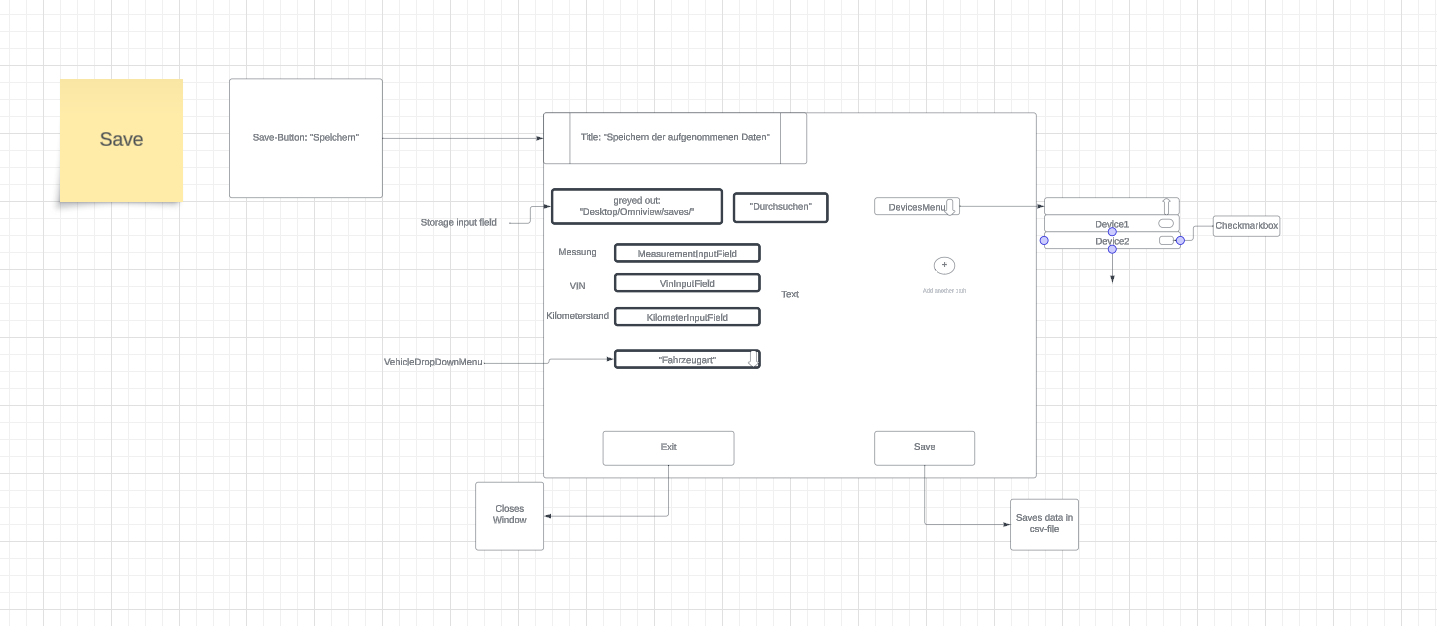
\includegraphics[width=.9\textwidth]{SaveandOpenLucidChartScreenshot.png}
    \caption[]{A visual representation of the saving process in the user interface}
    \label{fig:saveData}
\end{figure}

\subsubsection{load again button/reset button}

The reset button resets all measurements and reloads all connected devices.


\subsubsection{start and stop button states}

it is not clear at the moment if the start and stop button are included in the toolbar or the datawindow



\subsection{Datawindow}

The Datawindow is positioned in the middle of the screen. The size of the window changes when the devices list or the sidebar menu are opened or closed. The screensize should always take up the maximal available space. 
The Datawindow displays the choosen files and the current measured data. It also contains a legend where the devices and files are shown with their corresponding color. The legend can be opened and closed. 
The Datawindow is shown in figure \ref{fig: datawindow}.\\
\begin{figure}
    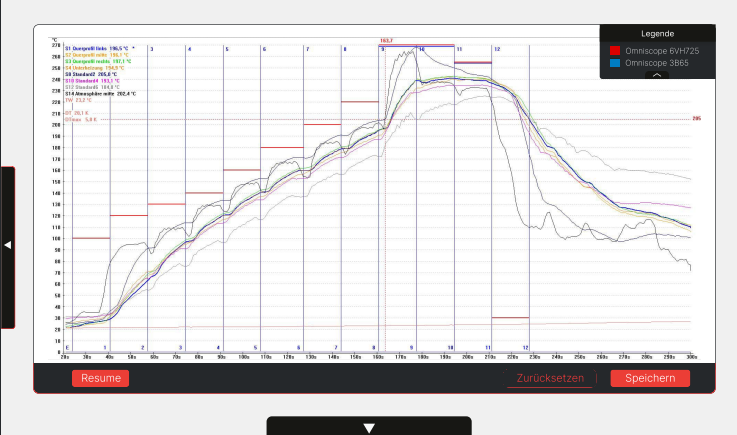
\includegraphics[width=.9\textwidth]{assets/pictures/DatawindowVersion1.0.png}
    \caption[]{A visual representation of the datawindow with a legend.}
    \label{fig: datawindow}
\end{figure}

Right now it is not decided if the start and stop buttons are placed in the toolbar or in the datawindow. \\

While a measurement is taken the datawindow cant be changed. While the measurement is taken, the software should automatically zoom in or out so the whole data on the y-axis is displayed and at least the last 10 seconds of the measurement on the x-axis. \\

After the measurement is finished the datawindow can be adjusted by the user. 

The following parts of the datawindow should be adjustable: 

\begin{itemize}
    \item zoom in and out on both axis
    \item scale of the x- and y-axis 
    \item choosing a part of the datawindow and only displaying this part 
\end{itemize}

The adjustments should be able to be made per mouse, mousepad, touchpad and with shortcuts. They also should be able to be set to a specific number. 
The user should be able to zoom in the dataset and cut out a specific part of the data. The image of the data should be able to be converted into a PDF by clicking the button "PDF" in the datawindow. 


\subsection{Side Bar Menu}

The side bar menu is positioned at the left side of the application. It can be extended and closed via a side button as shown in figure \ref{fig: sidebarMenu}. 
\begin{figure}
    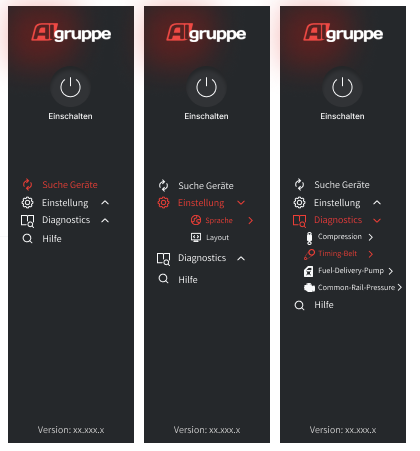
\includegraphics[width=.9\textwidth]{assets/pictures/SideBarMenu.png}
    \caption[]{A visual representation of the sidebar Menu in its different states}
    \label{fig: sidebarMenu}
\end{figure}
The menu contains five submenus:
\begin{itemize}
        \item searching devices named "Suche Geräte"
        \item loading old data named "Daten hinzufügen"
        \item Diagnostics named "Diagnose"
        \item Settings named "Einstellungen"
        \item Help named "Hilfe"
    \end{itemize}
Every Menu has their own icon. 
In the following the different devices are described.

\subsubsection{Searching devices}

The searching devices submenu is only defined by a button, shown in figure \ref{fig: sidebarMenu}. If the user clicks the button the Software will search for connected devices. If the connected devices are found they are shown in the device list menu. 
If OmniScopes are connected their light is switched to light blue. 

\subsubsection{Loading old data}

The loading old data menu is also a button shown in figure \ref{fig: sidebarMenu}. If the button is clicked the "Load old data" Popup window is shown. 
The configurations for this Popup window can be found in the section \ref{cap: PopupWindow_loadoldata}.
After making the configurations the loaded data is also shown in the devices list and the datapoints are shown in the Datawindow.


\subsubsection{Diagnostics menu}

The Diagnostics menu is a drop down menu as shown in figure \ref{fig: sidebarMenu}. 
The first layer contains the different possible analyses the user can make. The second layer contains the option "Analysiere Daten" (analyse current waveform) and "Generiere Trainingsdaten" (generate Trainingsdata). If one of the options is selected the associated PopupWindow is openend.
For "analyse current waveform" the associated PopupWindow description can be found in \ref{cap: PopupWindow_analysedata}, the other PopupWindow description can be found in \ref{cap: PopupWindow_generate_training_data}.

\subsubsection{Settings menu}

The settings menu is a drop down menu as shown in figure \ref{fig: sidebarMenu}. 
The first layer contains the buttons
\begin{itemize}
    \item Sprache (language)
    \item Layout 
    % \item ligth and dark mode 
\end{itemize}

When clicking the language button a second drop down menu opens where the user can select the language via a click on the language name. 
When clicking on the Layout button the "layout" popupwindow described in the section \ref{cap: PopupWindow_layout} appears. 

\subsubsection{Help menu}

The help button is a button that leads to a website. Before the user access the website a popup window appears that ask the user if he wants to be lead to the website or not. 


\subsection{PopupWindows}
This section describes the configuration of the different PopUpWindows and their functionality.

\subsubsection{PopupWindow: Layout}\label{cap: PopupWindow_layout}


\subsubsection{PopUpWindow: Load old data}\label{cap: PopupWindow_loadoldata}
The load old data window should have two options: 
\begin{itemize}
    \item entering a file by typing in a path or searching through the file system
    \item entering a file by a drag and drop field 
\end{itemize}
For the first option there is a input field with a "Durchsuchen" (searching) button on the top half of the popupwindow. When clicking the searching button the file system opens and the user can choose a file.
For the second option there is a drag and drop field on the bottom half of the popupwindow with the description "Datei einfügen" (drop file). 


\subsubsection{PopupWindow: analyse data}\label{cap: PopupWindow_analysedata}

The analyse data window is build with the same structure as the generate training data popupwindow. A picture is shown in figure \ref{fig: analysedata Popupwindow}. 
The first half of the menu including the measurement, VIN and mileage inputfields the functionality of the buttons is the same, except that the user can choose more than one file to be analysed. The main difference is in the bottom half of the menu, this menu has three stages. 
\begin{itemize}
    \item before starting the analysis 
    \item during the analysis
    \item after the analysis
\end{itemize}

\textbf{Before the analysis}: 
Before the analysis starts the user can only click on two buttons "Abbrechen"(cancel) which closes the window and "Analysiere"(analyse) which starts the analysis. When the analyze is started the chosen data will be send to a AP which is connected to a different device where the analysis is running. \\

\textbf{During the analysis}
During the analysis the menu shows a loading bar in the bottom half and the options are greyed out except the cancel button. The user can still cancel the analysis at any given time. 
The loading bar is shown because an analysis can take a lot of time. While the analysis is running the user can minimize the window but cant close it. He can use the application in any way and also can run two or more analyses at the same time.\\

\textbf{After the analysis}
After the analysis the user gets a message via a popup window that his analysis is finished. In the menu he can now see the different datasets he analyzed on the left side and the results in the middle. 
The results are displayed via a up or down thump in green or red. On the right side the user finds a redname that is clickable. If he clicks on the name a PDF where his measurement is displayed and the test results with a explanation under the picture of the measurement are displayed. The user can download this PDF in the given PDF viewer.  



\subsubsection{PopupWindow generate training data}\label{cap: PopupWindow_generate_training_data}

\textbf{General structure of the "Generate training data" menu.} 

The "generate training data" PopUpwindow pops up if the user clicks on one of the "generate training buttons" that are found under "Diagnostics" -> Analysetype (for example "Compression") -> "generate training data". The generate training data window is designed after the design principle for Popupwindows found in \ref{cap:Designprinciples_Popupwindows} and is shown in figure \ref{fig: Generate Training data Popupwindow}.\\  In the upper third it contains two Radio Buttons. I the middle there are a ID,VIN and MILEAGE field and three Radio Buttons with the title "Reason-for-investigation", "Electrical Consumers" and "Assessment". In the bottom third there is a comments Input-field and in the right corner a cancel and send button. 

\begin{figure}
    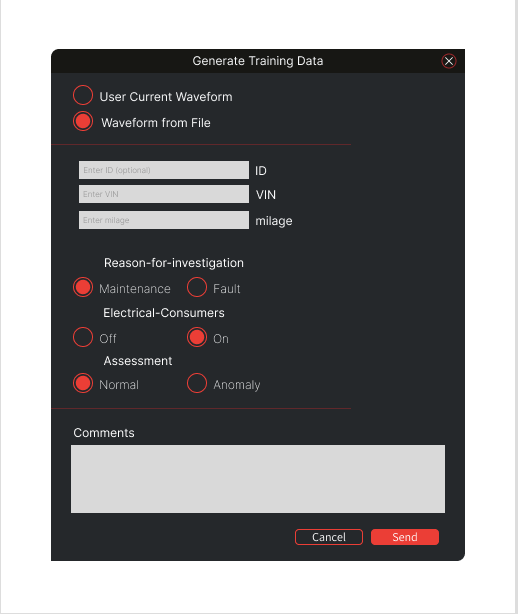
\includegraphics[width=.9\textwidth]{assets/pictures/GenerateTrainingDataMenu.png}
    \caption[]{A visual representation of the "Generate Training data" Popup window}
    \label{fig: Generate Training data Popupwindow}
\end{figure}

\textbf{Functionality of the "Generate Training data menu"}

Generally, the PopupWindow 'Generate Training Data' is used to send measured waveform stacks to an API, where the data is sent to a KI. This data is used for training the KI model.

To choose the data to be sent, the user has two options selectable by the Radio Buttons 'Use a Current Waveform' or 'Use Waveform from File'.

By choosing the first option, a drop-down menu appears, displaying the connected device and loaded data. It is designed following the design principle \ref{cap:Designprinciples_dropDownMenusWithCheckmark}. 
The user can choose which device or loaded data (waveform) to send by clicking the checkbox next to the device or loaded data. The user can only send one waveform.

By choosing the second option, a drag-and-drop area for selecting a file from the PC's storage appears under the 'Waveform from File' Radio Button. 
All elements under the 'Waveform from file' button should be rearranged to accommodate the space occupied by the drag and drop field. 
The user can only input a file of type '.csv' from the storage. If they try to input another file format, the warning message 'Wrong format' should pop up. 
Once the user successfully uploads the file, the filename will be displayed in the drag-and-drop field, providing confirmation that the file has been accepted.

Under the 'Use waveform from file' field, there are three input fields for the ID, VIN, and mileage. The ID should be read from the config file. 
If it hasn't been set yet, the message 'Set your ID in settings' should appear greyed out in the field. The user can only set the ID in the settings menu. For the VIN and Mileage, the following should be used:
\begin{itemize}
    \item If the user already saved the current measurement, the fields should automatically be filled with the data the user put into the fields from the save PopupWindow.
    \item If the user used the second option or chose a 'loaded data file' in the first option, the VIN and mileage should automatically be read from the header of the CSV file and put into the VIN and mileage fields.
    \item If the user neither chose old data nor saved the data before, the user has to put in the VIN and mileage by themselves.
\end{itemize}

If the ID, VIN, and Mileage have been loaded automatically, they should not be editable anymore. The ID, VIN, and mileage fields should be greyed out, and the user can't change the data anymore.

After choosing the right waveform stack, the user can configure different settings by the Radio Buttons (\ref{cap:Designprinciples_PopupWindowButtons}):
\begin{itemize}
    \item 'Grund der Aufnahme': 'Wartung' / 'Fehler' (Reason for investigation: Maintenance / Fault)
    \item Electrical Consumers: Off / On
    \item 'Bewertung': 'normal' / 'anormal' (Assessment: normal / anomaly)
\end{itemize}

In the last field, the user can add a comment.

All options should be saved in a message, which is sent along with the data to the API.

At the bottom of the menu, the user can either cancel the configuration via the 'Abbrechen' (Cancel) button or send the data via the 'Senden' (Send) button.
 When pressing 'Cancel', the menu closes, and the old settings are deleted. When pressing 'Send', the data and the message are checked for the right format; otherwise, the user gets an error message, 
 and the sending process is canceled. If the check is positive, the data and message will be converted to a JSON string and sent to the API for the Analysetype individual with the correct API requirements. 
 If the data has been sent correctly, the message 'Your data has been sent' should pop up.
 If the API sends an error, the user should get the error message as a popup. The 'Send Training Data' counter in the config increments upon successful data transmission.

 \section{Elementdefintion}

\subsection{What is a Radio Button?}\label{cap:RadioButton}

A radio button, in the context of user interface design and interaction, is a graphical control element that allows users to choose one option from a set of mutually exclusive options. 
It typically appears as a small circular or round button that can be either selected (checked) or deselected (unchecked). 
When one radio button in a group is selected, any other radio buttons in the same group are automatically deselected.

The term "radio button" is derived from the similarity to the preset station buttons on older car radios, where pressing one button would cause any previously pressed button to pop out,
 indicating the selection of a specific station. Similarly, in a graphical user interface, selecting one radio button deselects any previously selected radio button in the same group. 
 This behavior is useful when users need to make a single choice from a list of options.



\section{Design Principles}\label{cap:Designprinciples}

\subsection{Design of Popupwindows}\label{cap:Designprinciples_Popupwindows}

\subsubsection{Design of Buttons in PopupWindows}\label{cap:Designprinciples_PopupWindowButtons}

\subsection{Design of Icon Buttons}\label{cap:Designprinciples_IconButtons}

\subsection{Design of a Drop Down Menu with checkmarks}\label{cap:Designprinciples_dropDownMenusWithCheckmark}



%\subsection{Data upload window}

%The upload window should be an extra window that does not overlap with the datawindow. It should contain an upload button and an exit button. The user should be able to put in the 
%current dataset or another dataset from their database. 
%The window should contain fields where the user can put in 
%\begin{itemize}
%    \item the analysis type
%    \item the base data like the workplace of the measurement
%    \item the reasons for the measurement
%    \item if the measurement shows expected course or not 
%\end{itemize}



%\subsection{Help menu}

%The Helpmenu should contain 
%\begin{itemize}
%    \item a link to our ous
%    \item a link to an Tutorial website
%\end{itemize}


\printglossaries

\end{document}

